%++++++++++++++++++++++++++++++++++++++++
% Don't modify this section unless you know what you're doing!
\documentclass[letterpaper,12pt]{article}
\usepackage{tabularx} % extra features for tabular environment
\usepackage{graphicx} % takes care of graphic including machinery
\graphicspath{ {./images/} }
\usepackage[margin=1in,letterpaper]{geometry} % decreases margins
\usepackage{cite} % takes care of citations
\usepackage{float}
%++++++++++++++++++++++++++++++++++++++++


\begin{document}

\begin{titlepage} % Suppresses displaying the page number on the title page and the subsequent page counts as page 1
	\newcommand{\HRule}{\rule{\linewidth}{0.5mm}} % Defines a new command for horizontal lines, change thickness here
	
	\center % Centre everything on the page
	
	%------------------------------------------------
	%	Headings
	%------------------------------------------------
	
	\textsc{\LARGE Advanced User Interface}\\[0.5cm] % Main heading such as the name of your university/college
	
	\textsc{\Large 2018/19}\\[0.5cm] % Major heading such as course name
	
	%------------------------------------------------
	%	Title
	%------------------------------------------------
	
	\HRule\\[0.4cm]
	
	{\huge\bfseries Public speech in Virtual Reality}\\[0.4cm] % Title of your document
	
	\HRule\\[1cm]
	
	
	\large\textit{Author}\\[0.3cm]
	Alberto Patti\\
	Lorenzo Salerno\\
	Zhu Yu\\[1.5cm]
	

	\begin{abstract}
	\end{abstract}
	\begin{table}[h]
		\centering
		\begin{tabular}{|l|l|l|l|}
			\hline
 			& Alberto Patti & alberto.patti@mail.polimi.it & 3389594345\\ \hline
 			& Lorenzo Salerno & & \\ \hline
 			& Zhu Yu & & \\ \hline
		\end{tabular}
	\end{table}
\end{titlepage}

\tableofcontents
\pagebreak
\section{Introduction}
	\subsection{Purpose}
The purpose of this document is to give information about the "WIVR games for stress relief" project developed for the Advanced User Interface course.\\
This document aims to explain:
\begin{itemize}
	\item The needs, goals and requirements for the targeted users;
	\item Previous researches and projects on the same topic;
	\item The choices made throughout the development of the project;
\end{itemize}

\subsection{Scope}
"Public speech in Virtual Reality" (SpeechVR) is a VR application that tries to give an instrument to people that have fear of speaking in public to improve their ability to speak to an audience.\\
The application offers to the user a virtual theatre where he/she can try a speech in front of an audience that can react based on his/her performance. The main functionality of the application is given by a biosensor (Empatica E4) that allows the tracking of the heart rate and the galvanic skin response of the user to evaluate the state of mind of the subject and decide how the environment should change: whether thee amount of people that the user sees in the audience can be changed or, in case the application consider that the user is in a situation of high stress, block the test.
 
\subsection{Definitions, acronyms and abbreviations}
\begin{itemize}
	\item VR: Virtual Reality
	\item HMD: Head Mounted Display
	\item WIVR: Wearable Immersive Virtual Reality
	\item HR: Heart Rate
	\item GSR: Galvanic Skin Response
\end{itemize}

	\pagebreak

\section{NGR}
	\subsection{Target}
The main target of the project are people that have fear of speaking in public. This kind of fear can be categorized as part of social phobia, i.e. "persistent fears of situations involving social interaction or social performance or situations in which there is the potential for scrutiny by others"\cite{model}.

\subsection{Context and Needs addressed}
"In social/evaluative situations, the primary threat stimulus is an audience and the primary threatening outcome is negative evaluation from the audience"\cite{model}.
The idea of being evaluated by the audience is enough to start a loop that keeps fueling the anxiety of the subject as shown in figure \ref{fig:model}.
\begin{figure}[!h]
	\centering
	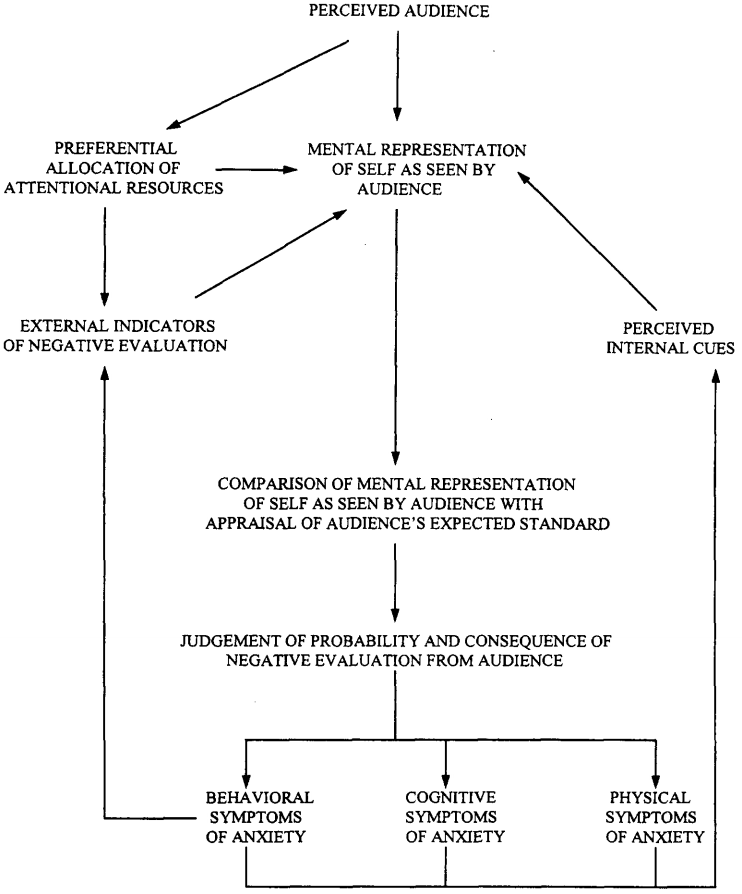
\includegraphics[scale=0.55]{Model}
	\caption{A model of the generation and maintenance of anxiety in social/evaluative situations\cite{model}.}\label{fig:model}
\end{figure}

For this reason the needs that were formulated are:
\begin{itemize}
	\item Have more confidence around people during the speech
	\item Listen to the speech after the performance
\end{itemize}

\subsection{Constraints}
\begin{itemize}
	\item HMD;
	\item A smartphone running Android Jellybean or higher (4.1.x+);
	\item Empatica E4;
	\item Microphone;
	\item Headphones;
	\item A pc (Windows 7 or higher) with Visual C++ Redistributable Package installed
	\item Bluegiga Bluetooth Smart Dongle
	\item Comfortable place where the user can sit down and rest the arm
\end{itemize}

\subsection{Goals}
\begin{itemize}
	\item Improve the ability to speak in public
	\item Allow the subject to be less anxious before and during the speech
\end{itemize}

\subsection{Requirements}

\begin{itemize}
	\item The applications should provide an environment where the subject can try his/her speech in front of a virtual audience.
	\item The application should progressively change the number of people that the user can see in the audience based on his/her state of mind.
	\item The application should calm the subject if needed.
	\item The application must stop the test in case the subject doesn't feel well.
	\item The application should reward the user on a good performance.
	\item The application should record the speech and play it if needed.
\end{itemize}





	\pagebreak
	
\section{State of the art}
	\subsection{Applications}
There are many application with the same target and objectives as this project that were developed and are nowadays available:
\begin{itemize}
	\item Virtual Orator
	\item Speech Center VR
	\item VirtualSpeech
	\item \#BeFearless
	\item Public Speaking Simulator VR
\end{itemize}
These are some of the available applications but, even though the premises are the same, each of them present different features and are available on different platform as shown in the tables below.

{
\renewcommand{\arraystretch}{1.3}
\begin{table}[H]
	\centering
	\begin{tabular}{|l|l|l|}
		\hline
		Virtual Orator & Oculus Rift / HTC Vive & 3D Environment\\ \hline
		Speech Center VR & Oculus Rift & 3D Environment\\ \hline
		VirtualSpeech & Android & 360° video\\ \hline
		\#BeFearless & Android & 3D Environment\\ \hline
		Public Speaking Simulator VR & Android & 3D Environment\\ \hline
	\end{tabular}
\end{table}
} 
{
\renewcommand{\arraystretch}{1.5}
\begin{table}[H]
	\centering
	\begin{tabular}{l|c|c|c|c|c|c|c|c|c|c|}
		\cline{2-11}
 		& \multicolumn{1}{l|}{\rotatebox{270}{Multiple Environment}} & \multicolumn{1}{l|}{\rotatebox{270}{Upload documents}} & \multicolumn{1}{l|}{\rotatebox{270}{Record your performance}}
 		& \multicolumn{1}{l|}{\rotatebox{270}{Question from the audience}} & \multicolumn{1}{l|}{\rotatebox{270}{Speech analysis}} & \multicolumn{1}{l|}{\rotatebox{270}{Distractions}}
 		& \multicolumn{1}{l|}{\rotatebox{270}{during the speech} \newline \rotatebox{270}{Variable number of people} } & \multicolumn{1}{l|}{\rotatebox{270}{Biosensor}}
 		& \multicolumn{1}{l|}{\rotatebox{270}{Lectures}} & \multicolumn{1}{l|}{\rotatebox{270}{Evaluation of the performance }} \\ \hline
		
		\multicolumn{1}{|l|}{Virtual Orator} & X & X & X & X &  & X &  &  &  &  \\ \hline
		\multicolumn{1}{|l|}{Speech Center VR} & X & X & X &  &  & X &  &  & X & X \\ \hline
		\multicolumn{1}{|l|}{VirtualSpeech} & X & X & X &  & X & X &  & X & X & X \\ \hline
		\multicolumn{1}{|l|}{\#BeFearless} & X & X & X &  & X &  &  & X &  & X \\ \hline
		\multicolumn{1}{|l|}{Public Speaking Simulator VR} &  &  &  &  &  & X & X &  &  &  \\ \hline
	\end{tabular}
\end{table}
}
The base of this project is the same as the application listed before: giving the user an environment where he/she can freely try his/her speech. What makes SpeechVR unique is the usage of a biosensor as a mean to control the environment the user is put in. In fact, the only app that uses a biosensor are VirtualSpeech and \#BeFearless but they use it as another parameter to give a score to the overall performance.

\subsection{Research}
There are many researches about public speech anxiety (and social phobia in general) but the most relevant for the sake of this project are:

\begin{itemize}
	\item Slater, M., Pertaub, D. P., \& Steed, A. (1999). Public speaking in virtual reality: Facing an audience of avatars.\cite{VRPublicSpeaking}\\[0.15cm]
	The focus of this paper is to analyze how people evaluate themselves while in front of an audience with different reactions using VR.
	
	\item Pertaub, D. P., Slater, M., \& Barker, C. (2002). An experiment on public speaking anxiety in response to three different types of virtual audience.\cite{VRPublicSpeaking2}\\[0.15cm]
	This is a more thorough analysis of the previous research.
	
	\item Chollet, M., Sratou, G., Shapiro, A., Morency, L. P., \& Scherer, S. (2014, May). An interactive virtual audience platform for public speaking training.\cite{VRPublicSpeaking3} \\[0.15cm]
	The focus of this research is to design a way to let people learn how to behave in front of a fake audience that reacts to the user actions. This research doesn't use VR but instead works with screens and audiovisual sensors (Kinect) to analyze the user behaviour.
	
	\item Poeschl, S., \& Doering, N. (2012, March). Virtual training for Fear of Public Speaking—Design of an audience for immersive virtual environments.\cite{VRPublicSpeaking4}\\[0.15cm]
	This research explains how to develop an audience that shows realistic behaviour.
	
	\item McKinney, M. E., Gatchel, R. J., \& Paulus, P. B. (1983). The effects of audience size on high and low speech-anxious subjects during an actual speaking task.\cite{VRPublicSpeaking5}\\[0.15cm]
	This research studies how people react during a speech in front of different amount of people hearing.
\end{itemize}
	\pagebreak
	
\section{UX design}

\section{Implementation}
	\subsection{Introduction}
The main application of the project is an Android app built on Unity. This allows the creation of a VR environment with ease. The only problem that arises from this choice is that it isn't possible to retrieve the data from the biosensor and send them to the smartphone directly as Unity doesn't allow a direct communication. As shown in figure \ref{fig:communication} the information from the biosensor are read first by a Computer and then sent to a Firebase server that stores the values. This values are then read by the Android application using a HTTP request.
\begin{figure}[h]
	\centering
	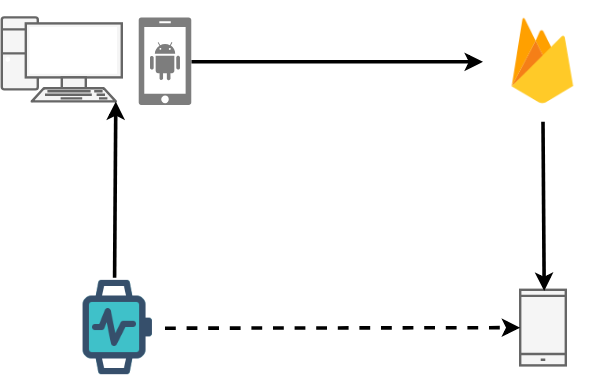
\includegraphics[scale=0.7]{ConnectionDiagram}
	\caption{Diagram that shows how the communication from the biosensor to the smartphone works.}\label{fig:communication}
\end{figure}

\subsection{Android Application}
Language used: C\#\\
Plugins:
\begin{itemize}
	\item ZXing
	\item Android Runtime Permissions
\end{itemize}

\subsection{Computer Client}
Language used: Java
Plugins:
\begin{itemize}
	\item ZXing
	\item JavaFX
\end{itemize}

	\pagebreak
	
\section{Value proposition}

\section{Future work}


%++++++++++++++++++++++++++++++++++++++++
% References section will be created automatically 
% with inclusion of "thebibliography" environment
% as it shown below. See text starting with line
% \begin{thebibliography}{99}
% Note: with this approach it is YOUR responsibility to put them in order
% of appearance.

\begin{thebibliography}{99}

\bibitem{model}
Rapee, R. M., \& Heimberg, R. G. (1997). A cognitive-behavioral model of anxiety in social phobia. Behaviour research and therapy, 35(8), 741-756.

\end{thebibliography}


\end{document}